%%% what LGADs are
%%% working principles
%%% requirements for the detector
%%% other studies 
%%% expected results
\chapter{HGTD and LGADs}\label{chap:HGTD_LGADs}

%%% I have to put an actual "summary" of the chapter
% In this chapter we motivate the construction of HGTD, illustrate its general layout and describe the specific type of silicon sensors (LGADs) that constitute the active components of the detector.
The upcoming High-Luminosity phase has the goal of increasing the integrated luminosity by a factor \(10\), enhancing the potential of new physics discoveries. However, it will also bring a variety of new complications, most importantly the increase in pileup interactions\footnote{Multiple collisions happening during the same bunch crossing, on top of a main event of interest.}.
%%% HGTD as a solution 
A new way to mitigate this effect for higher pseudorapidity values will be "\textit{to use high-precision timing information to distinguish between collisions occurring very close in space but well-separated in time}" \cite{CERN-LHCC-2020-007}. This is set to be accomplished by the High Granularity Time Detector (HGTD).
The HGTD will improve the object reconstruction capabilities of ATLAS, complementing ITk. This, in turn, will help study a variety of processes that rely on the precise identification and measurement of the physics objects produced during \(p-p\) collisions, such as jets and leptons.
The detector's active elements will be silicon sensors, which will provide precise timing information and will withstand the additional radiation of the HL. To achieve the HGTD's preicison goal of \qty{30}{\pico\second} (\qty{50}{\pico\second}) at start life (end life), the sensors will need to have a time resolution per hit of \qty{35}{\pico\second} (\qty{70}{\pico\second}). Additionally, a hit efficiency above \(95\%\) and %a due to the electronics' spefications,
a minimum collected charge of \qty{4}{\femto\coulomb} will also be required.
% I need to add the sensor requirements: time resolution, charge and efficiency 

In this chapter we describe the general design of the HGTD, its benefits to object reconstruction and the special type of silicon sensors (LGAD) that will form its basic components.

\section{The High Granularity Time Detector}\label{sec:HGTD}
%%% ITk
One of the updates to the ATLAS detector will be the installation of the new ITk, which will improve the tracking\footnote{Tracking refers to the process of reconstructing the paths of charged particles as they fly through a detector. From the curvature of the track the momentum and the charge can be inferred. It is a fundamental part of event reconstruction.} and will extend the pseudorapidity range up to \(\eta=4\). While this extension will improve the reconstruction of physics objects, it will bring some difficulties too.

%%% event reconstruction
Event reconstruction relies strongly on the precise assignment of a track to the location of the first collision (primary vertex). % (track-to-vertex association).
Generally, a track is associated to a vertex if the track's origin is compatible with the vertex, this compatibility can be determined with:

\begin{equation}\label{eq:compatibility_vertex}
    \frac{\left|z_0 - z_{vertex}\right|}{\sigma_{z_0}} < s \,.
\end{equation}
 
Where \(z_0\) is the longitudinal impact parameter, \(z_{vertex}\) is the vertex position, \(\sigma_{z_0}\) is the spacial resolution and \(s\) is a significant cut (typically 2.5 or 3)\cite{cernTechnicalDesign}. 

\begin{figure}[h!tbpt]
    \centering
    \subfloat[Simulation of the local pileup vertex densities for two values of \(<\mu>\) (average number of collisions per bunch crossing), indicative of the current and future collision rates. From~\cite{cernTechnicalDesign}.]{
        \includegraphics[width=.45\linewidth]{Images/intro/pileup_density_simulation.png}
        \label{fig:pileup_densities}}
    \hfill
    \centering
    \subfloat[Simulation of the longitudinal resolution of ITk as a function of \(\eta\), for muons with \(p_T=\qty{1}{\giga\electronvolt}\) and \(p_T=\qty{10}{\giga\electronvolt}\) From~\cite{cernTechnicalDesign}.]{
        \includegraphics[width=.46\linewidth]{Images/intro/ITk_z_resolution_for_eta.pdf}
        \label{fig:ITk_spacial_resolution}}
    \caption{Simulations of the pileup densities (left) and the ITk spacial resolution (right).}
\end{figure}

%%% difficulties/problems
Some problems arise. 
Firstly, as \(\eta\) increases, tracks become more parallel to the beam and are subject to multiple scattering effects due to more material compared to the central barrel region. Secondly, the HL-LHC will see a rise in the number of collisions per bunch %\footref{footnote:particle_beam_bunches} %%% this footnote is from the previous chapter, so it gives the wrong number
 and, as a direct consequence, an increase in the average density of hard-scatter vertices (Figure~\ref{fig:pileup_densities}). Lastly, the resolution of ITk in the z direction (i.e. the beam direction) worsens considerably at higher pseudrapidities, as shown in the simulation in Figure~\ref{fig:ITk_spacial_resolution} for two values of \(p_T\)\footnote{\(p_T\) is the transverse momentum: the component of the momentum perpendicular to the beam line.}.

%%% check if I mention how these problems will be solved

%%% HGTD provides time measurements
The HGTD will provide time information of charged particles with a time resolution of 30ps (up to 50ps at the end of life). %This will enhance the physics capabilities of ATLAS in three main ways:
This will improve object reconstruction, for example of forward jets and leptons, which is key in many processes, like VBF (vector bosons fusion) and VBS (vector bosons scatter). % where interesting events must be separated from the background.

The most powerful way to utilise this timing information is to require each track to satisfy:

%%% time window compatibility (formula) t-t_0 / sigma < s
\begin{equation}
    \frac{t_{track}-t_0}{\sigma_t} < s \,.
\end{equation}

%%% other advantages
Where \(t_0\) is the time of the primary vertex, \(t_{track}\) is the time of the track, \(\sigma_t\) is the combined error and \(s\) is a significant cut, analogously to Eq~\ref{eq:compatibility_vertex}. % It should be noted, however that the experimental challenges of the determination of \(t_0\) will limit the full power of this approach \cite{cernTechnicalDesign}.
The detector will also introduce new timing information to the data, independent of other detector measurements. And finally, the HGTD will provide an additional, precise way to measure luminosity both online (instantanous, during operations) and offline (calculated after data taking), contributing to the ATLAS goal of 1\% uncertainty on luminosity, which is the largest source of uncertainty in many analyses, such as for precision measurements of the Higgs boson~\cite{CERN-LHCC-2020-007}.

% %%% I put these points above
% \begin{itemize}
%     \item Improving object reconstruction, for example forward jets and leptons, which is key in many processes, like VBF (vector bosons fusion) and VBS (vector bosons scatter).% where interesting events must be separated from the background.
%     \item Introducing new information based on timing measurements that is independent of other detectors.
%      %%% HGTD measures luminosity 
%     \item Providing an additional, precise way to measure luminosity both online (instanteous, during operations) and offline (calculated after data taking), contributing to the ATLAS goal of 1\% uncertainty on luminosity, which is the largest source of uncertainty in many analyses, such as for the Higgs boson~\cite{CERN-LHCC-2020-007}.
% \end{itemize}

%%% detector layout
% eta=2.4 -> theta=10.367°      eta=4 -> theta=2.0986°
The detector will cover pseudrapidities between \(2.4 < \eta < 4.0\) (so an incident angle roughly between 2° and 10°), complementing the ITk (Inner Tracker).
% picture of HGTD
\begin{figure}[h!tbpt]
    \centering
    \subfloat[The detector will be placed outside the volume of the future Inner Tracker, between the Barrel ande Forward Calorimeters]{
        \includegraphics[width=.6\linewidth]{Images/intro/HGTD_position_and_layout.png}
        \label{fig:HGTD_location}}
    \hfill
    \centering
    \subfloat[The overlap between modules on the front and the back was optimized to give an approximately uniform performance (as a function of radius) \cite{CERN-LHCC-2020-007}.]{
        \includegraphics[width=.35\linewidth]{Images/intro/HGTD_disks_alignment.png}
        \label{fig:HGTD_schema}}
    \captionsetup{width=\captionwidth}
    \caption{Location (left) of the HGTD inside ATLAS and orientation (right) of the two faces on each disk. From \cite{cernTechnicalDesign}.}
\end{figure}

%%% detector layout
The detector consists of two thin disks with that will be placed outside the ITk, as shown in Figure~\ref{fig:HGTD_location}. Each disk includes two instrumented double-sided layers, a hermetic vessel and two moderator pieces, inside and outside the vessel (to reduce the back-scattered neutrons created by the end-cap/forward calorimeters). The detector is further divided into three concentric active regions, as can be seen in Figures \ref{fig:HGTD_location} and \ref{fig:HGTD_schema}, ranging: \qty{120}{\milli\meter}-\qty{230}{\milli\meter}, \qty{230}{\milli\meter}-\qty{470}{\milli\meter} and \qty{470}{\milli\meter}-\qty{640}{\milli\meter} \cite{CERN-LHCC-2020-007}. Beyond the outer region are the peripheral electronics.
%%% the modules
The two disks are covered by 8032 modules in total, each module containing two silicon sensors and two ASICs (Application-Specific Integrated Circuit). Each sensor features 15x15 pads of Low Gain Avalanche Detectors (LGAD), a specific type of silicon sensors (\nameref{sec:LGADs}).

%%% radiation damage and replacement
The radiation that the components will withstand depends strongly on the radius. Due to electronics and sensors specifications, a minimum charge of \qty{4}{\femto\coulomb} is required. This is achievable up to a radiation damage level of \qty{2.5e15}{\neutroneq\centi\meter^{-2}} (neutron equivalent\footnote{The radiation damage equivalent to neutrons at \qty{1}{\mega\electronvolt}}); as a result, the sensor and electronics within the smallest ring will be replaced after each \qty{1000}{\femto\barn^{-1}} and the ones within the middle ring will be replaced at half of the data-taking (\qty{2000}{\femto\barn^{-1}}).


\section{Low Gain Avalanche Detectors}\label{sec:LGADs}

\marginpar{\flushleft Other image/photo of LGAD?}

A special type of silicon sensors were chosen as the active element for the HGTD. Due to their precision, limited thickness and internal gain.

\subsection{Working principles of silicon sensors}

The core of a silicon sensor consists of a junction between two differently doped layers (Figure~\ref{fig:p-n_junction_reverse_bias_voltage}), which means that small concentrations of impurities with either higher atomic number (donors, \(n\)-type) or lower (acceptors, \(p\)-type) are introduced inside the crystals.
This forms a \(pn\)-junction, and when a voltage is applied with positive potential on the \(n\)-side and negative on the \(p\)-side (reverse bias) the volume between the two layers is depleted of mobile charges, and it becomes an insulator with an internal electric field.

%%% Figure~WITH MINIPAGE (for side caption)
\begin{figure}[h!tbpt]
    \begin{minipage}[c]{.25\linewidth}
        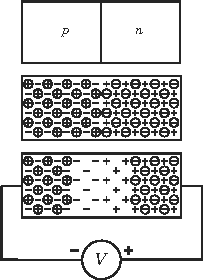
\includegraphics[width=1\linewidth]{Images/LGADs/p-n junction with voltage.png}
    \end{minipage}
    \hfill
    \begin{minipage}[c]{.6\linewidth}
        \caption{\\Top: adjacent regions of \(p\)-doping (left) and \(n\)-doping (right) forming a \(pn\)-junction.\\
        Middle: the circled mobile charges (holes for \(p\)-type and electrons for \(n\)-type) balanced by the charge of atomic cores.\\
        Bottom: when an external (reverse) voltage is applied to the junction, an electric field builds up in the central region, depleting it of free mobile charges \cite{10.1093/acprof:oso/9780198527848.003.0001}.}
        \label{fig:p-n_junction_reverse_bias_voltage}
    \end{minipage}
\end{figure} 

When a charged particle traverses this depletion layer it frees up electron-hole pairs, which move to the electrodes and can be observed as a pulse in the electric potential.
Silicon sensors generally offer several advantages over other type of detectors. The lower energy requirement to produce electron-hole pairs leads to improved energy resolution. Moreover, compared to gas detectors for example, silicon sensors have much higher density, allowing precise measurements in significantly thinner layers. However, this type of device has typically higher manufacturing costs and suffers more considerably from radiation damage.

\subsection{LGADs}

\begin{figure}[h!tbpt]
    \begin{minipage}[c]{.45\linewidth}
        \includegraphics[width=1\linewidth]{Images/LGADs/LGADs_schema_of_work.png}
    \end{minipage}
    \hfill
    \begin{minipage}[c]{.4\linewidth}
        \caption{Cutaway view of an LGAD, not to scale. The depletion region makes the majority of the volume of the sensor, and above it, lies the avalanche region. On the left of the picture there is a qualitative plot of the electric field along the vertical axis of the sensor, highlighting the strong electric field in the avalanche region. From \cite{cernTechnicalDesign}.}
        \label{fig:LGADs_schema}
    \end{minipage}
\end{figure} 

A particular type of silicon sensors are Low Gain Avalanche Detectors (LGAD), an illustration is shown in Figure~\ref{fig:LGADs_schema}. The major innovation over standard silicon sensors is an additional \(p\)-type layer below the \(n+\) electrode. This creates a high electric field region which leads to an avalanche effect\footnote[2]{When electrons acquire enough energy they can create new electron-hole pairs ('impact ionization'), which can themselves create new pairs and initialize a multiplication chain that leads to an enhanced signal} of the electrons. 
Charged particles in standard silicon produce roughly 65 e-h pairs per \unit{\micro\meter} of thickness \cite{meroli_energy_loss2011}, equivalent to around \qty{0.52}{\femto\coulomb} for \qty{50}{\micro\meter}. The avalanche effect magnifies the signal around 8-20 times (i.e. a \textit{gain} of 8-20), bringing the collected charge up to \qty{4}{\femto\coulomb}-\qty{10}{\femto\coulomb} \cite{cernTechnicalDesign}. % charged particle in 50 um of silicon produce ~0.52 fC of charge or 3280 e-h pairs

The intrinsic multiplication in LGADs amplifies the signal, improving the signal-to-noise ratio (S/N) and mitigating the signal degradation caused by radiation-induced noise.

The key metrics of the sensors are: time resolution, collected charge and efficiency.

\subsubsection{Time Resolution}

To accomplish a time resolution per track of \(\approx\qty{30}{\pico\second}\) (start) and \(\approx\qty{50}{\pico\second}\) (end), the sensors will require a time resolution per hit of \(\approx\qty{35}{\pico\second}\) (start) \(\approx\qty{70}{\pico\second}\) (end) \cite{CERN-LHCC-2020-007}.

Three major effects determine the time resolution of the sensors: time walk from amplitude variations\footnote{Time walk refers to the variation in signal timing caused by pulses with different amplitudes reaching a fixed threshold at different times.}, electronic noise jitter, and Landau fluctuations from charge deposition non-uniformities. 
\marginpar{\flushleft The plot of time walk effect }

\begin{equation}\label{eq:time_resoltuion_LGADs}
    \sigma^2 = \sigma_{TimeWalk}^2 + \sigma_{Jitter}^2 + \sigma_{Landau}^2  \, .
\end{equation}

 Both time walk and noise jitter depend on the type of readout electronics and depend inversely on the signal slope \(dV/dt\).

\begin{itemize}
    \item \(\sigma_{TimeWalk} = \left[ \frac{V_{th}}{S/t_{rise}}\right]_{RMS}\) where \(V_{th}\) is the threshold voltage, S is the signal (proportional to the gain) and \(t_{rise}\) is the time taken by a signal to go from 10\% to 90\% of the maximum amplitude.
    \item \(\sigma_{Jitter} = \frac{N}{dV/dt} \approx \frac{t_{rise}}{S/N}\) where \(S/N\) is the signal-over-noise ratio.
    \item \(\sigma_{Landau}\) depends on the thickness of the sensor (thinner is better) and the setting of the threshold voltage.
\end{itemize}

It can be noticed that the lowest jitter and time walk errors are achieved with high S/N and small rise time, i.e. thin sensors with high gain. Time walk can also be corrected with reconstruction algorithms, such as constant-fraction-discrimination (CFD), Figure~\ref{fig:constant fraction}.

\begin{figure}[h!btp]
    \centering
    \includegraphics[width=.8\linewidth]{Images/methods/Constant_fraction_1.pdf}
    \captionsetup{width=\captionwidth}
    \caption{Illustration of the \textit{time walk} effect: two pulses with similar shapes, but different amplitudes, can have distinct Time Of Arrivals. Two reconstruction algorithms are compared: Constant Threshold Discriminator (left) and Constant Fraction Discriminator (right). CTD has a fixed threshold value, so the TOA \(t\) is set when the pulse crosses the threshold. For CFD, the time \(t\) corresponds to the moment the pulse reaches a certain fraction of the maximum amplitude, removing the time walk effect.}
    \label{fig:constant fraction}
\end{figure} 


\subsubsection{Radiation damage}

Due to the harsh environment the sensors will be placed in, they will suffer significant damage caused by the extreme flux of highly energetic particles. At the microscopic level, this will cause irregularities in the silicon lattice, altering the bulk and surface properties. At the macroscopic level, there will be an increase in leakage current, a degradation in charge collection efficiency and a change in the effective doping concentration \cite{Moll:1999kv} (as the defects can behave as donors or acceptors). The leakage current can be sufficiently quenched by operating at low temperatures, the charge collection can be improved by applying higher bias voltages. But the last effect has the most detrimental impact on the properties of the sensors, which will deteriorate as the radiation dose increases.


\subsection{Signal generation by charged particles}\label{subsec:charged_particles_distribution}
%%% To find the gain of the sensors we have to first look at the charge deposited on a normal silicon sensor (without gain).
The theoretical probability distribution of the energy loss of heavy particles hitting a thin target (such as the active volume of a silicon sensor) has been solved rigorously by Vavilov in \cite{vavilov_1957}. The namesake distribution is a generalization of the Landau distribution, but its evaluation is more difficult, as it is expressed as an integral over some complicated functions \cite[Eq.(4)]{vavilov_1957}. Fortunately, it can be approximated by more straightforward functions depending on the value of a parameter \(\kappa\) (for a more detailed explanation see \ref{sec:vavilov_vs_landau_distribution}): for \(\kappa\rightarrow0\) the Vavilov distribution can be approximated by a Landau, for \(\kappa>>1\) by a Gaussian.

For the conditions of the tests studied in this thesis \(\kappa\approx \num{1e-8}\), well below the limit, thus the Landau function is a good approximation. It can be expressed by \cite{KOLBIG198497}:

\begin{equation}\label{eq:landau}
    \Phi (\lambda) = \frac{1}{\pi} \int_{0}^{\infty} e^{-\lambda u} u^{-u} \sin (\pi u ) \mathrm{d}u \, .
\end{equation}

Additionally, due to a combination of theoretical corrections \cite{PhysRevA.11.1286} (due to the atomic binding of the electrons) and statistical errors on the measurements, the final distribution of energy deposit follows more accurately the convolution of a Gaussian and a Landau distributions (Figure~\ref{fig:langau_convolution_plot}).

\begin{figure}
    \centering
    \includegraphics[width=.6\linewidth]{Images/LGADs/Landau_Gauss_convolution.png}
    \captionsetup{width=\captionwidth}
    \caption{Plot of Landau function (in blue) and the Landau x Gaussian convolution (in red), with equal Landau parameters and arbitrary units, both normalized to 1.}
    \label{fig:langau_convolution_plot}
\end{figure}

